\documentclass[a4paper,11pt]{article}
\usepackage{amsmath,amsthm,amsfonts,amssymb,amscd,amstext,vmargin,graphics,graphicx,tabularx,multicol} 
\usepackage[francais]{babel}
\usepackage[utf8]{inputenc}  
\usepackage[T1]{fontenc} 
\usepackage{pstricks-add,tikz,tkz-tab,variations}
\usepackage[autolanguage,np]{numprint} 
\usepackage{calc}

\setmarginsrb{1.5cm}{0.5cm}{1cm}{0.5cm}{0cm}{0cm}{0cm}{0cm} %Gauche, haut, droite, haut
\newcounter{numexo}
\newcommand{\exo}[1]{\stepcounter{numexo}\noindent{\bf Exercice~\thenumexo} : }
\reversemarginpar

\newcommand{\bmul}[1]{\begin{multicols}{#1}}
\newcommand{\emul}{\end{multicols}}

\newcounter{enumtabi}
\newcounter{enumtaba}
\newcommand{\q}{\stepcounter{enumtabi} \theenumtabi.  }
\newcommand{\qa}{\stepcounter{enumtaba} (\alph{enumtaba}) }
\newcommand{\initq}{\setcounter{enumtabi}{0}}
\newcommand{\initqa}{\setcounter{enumtaba}{0}}

\newcommand{\be}{\begin{enumerate}}
\newcommand{\ee}{\end{enumerate}}
\newcommand{\bi}{\begin{itemize}}
\newcommand{\ei}{\end{itemize}}
\newcommand{\bp}{\begin{pspicture*}}
\newcommand{\ep}{\end{pspicture*}}
\newcommand{\bt}{\begin{tabular}}
\newcommand{\et}{\end{tabular}}
\renewcommand{\tabularxcolumn}[1]{>{\centering}m{#1}} %(colonne m{} centrée, au lieu de p par défault) 
\newcommand{\tnl}{\tabularnewline}

\newcommand{\trait}{\noindent \rule{\linewidth}{0.2mm}}
\newcommand{\hs}[1]{\hspace{#1}}
\newcommand{\vs}[1]{\vspace{#1}}

\newcommand{\N}{\mathbb{N}}
\newcommand{\Z}{\mathbb{Z}}
\newcommand{\R}{\mathbb{R}}
\newcommand{\C}{\mathbb{C}}
\newcommand{\Dcal}{\mathcal{D}}
\newcommand{\Ccal}{\mathcal{C}}
\newcommand{\mc}{\mathcal}

\newcommand{\vect}[1]{\overrightarrow{#1}}
\newcommand{\ds}{\displaystyle}
\newcommand{\eq}{\quad \Leftrightarrow \quad}
\newcommand{\vecti}{\vec{\imath}}
\newcommand{\vectj}{\vec{\jmath}}
\newcommand{\Oij}{(O;\vec{\imath}, \vec{\jmath})}
\newcommand{\OIJ}{(O;I,J)}


\newcommand{\reponse}[1][1]{%
\multido{}{#1}{\makebox[\linewidth]{\rule[0pt]{0pt}{20pt}\dotfill}
}}

\newcommand{\titre}[5] 
% #1: titre #2: haut gauche #3: bas gauche #4: haut droite #5: bas droite
{
\noindent #2 \hfill #4 \\
#3 \hfill #5

\vspace{-1.6cm}

\begin{center}\rule{6cm}{0.5mm}\end{center}
\vspace{0.2cm}
\begin{center}{\large{\textbf{#1}}}\end{center}
\begin{center}\rule{6cm}{0.5mm}\end{center}
}



\begin{document}
\pagestyle{empty}
\titre{Exercices bilan : Volumes et géométrie dans l'espace}{}{}{4ème}{}

\vspace*{0.5cm}
\exo  \\
Afin de faciliter l'accès à sa piscine, Monsieur Joseph décide de construire un escalier constitué de deux prismes superposés dont les bases sont des triangles rectangles. Voici ses plans :\\


\bmul{2}

\includegraphics[scale=0.85]{volfigure3.eps} \\

\columnbreak

\textbf{Information 1} :\\

 Volume du prisme = aire de la base $\times$ hauteur ;\\
 
  $1 L = 1 dm^{3}$ \\


\emul

\textbf{Information 2} : Voici la reproduction d'une étiquette figurant au dos d'un sac de ciment de 35 kg.\\
 
\begin{center}
\includegraphics[scale=1.2]{volfigure4.eps} \\
\end{center}

\textbf{Questions} :\\

\q Démontrer que le volume de l'escalier est égal à 1,262 08 $m^{3}$. \\

\q Sachant que l'escalier est un ouvrage en béton courant, déterminer le nombre de sacs de ciment de 35 kg nécessaires à la réalisation de l'escalier.\\

\q Déterminer la quantité d'eau nécessaire à cet ouvrage.\\

\newpage

\vspace*{0.75cm}
\exo\\
Une maison est composée d'une partie principale qui a la forme d'un pavé droit ABCDEFGH surmonté d'une pyramide IABCD de sommet I et de hauteur [IK1] perpendiculaire à la base de la pyramide.\\

Cette pyramide est coupée en deux parties :\\
- une partie basse ABCDRTSM destinée aux chambres ;\\
- une partie haute IRTSM réduction de hauteur [IK2] de la pyramide IABCD correspondant au grenier.\\

On a : EH = 12 m ; AE = 3 m ; HG = 9 m ; IK1 = 6,75 m et IK2 = 4,5 m.\\
\textit{La figure donnée n'est pas à l'échelle.}

\begin{center}
\includegraphics[scale=0.8]{brevtexo.eps} 
\end{center}

\initq \q Calculer la surface au sol de la maison.\\

\q Des radiateurs électriques seront installés dans toute la maison, excepté au grenier. On cherche le volume à chauffer de la maison.\\
On rappelle que le volume d'une pyramide est donné par : $ V = \dfrac{B \times h }{3} $\\

\initqa \qa Calculer le volume de la partie principale.\\

\qa Calculer le volume des chambres.\\

\qa Montrer que le volume à chauffer est égal à 495 $m^{3}$.\\

\q Un expert a estimé qu'il faut dans cette maison une puissance électrique de 925 watts pour chauffer 25 mètres cubes.\\
Le propriétaire de la maison décide d'acheter des radiateurs qui ont une puissance de 1 800 watts chacun et qui coûtent 349,90 euros pièce.\\
\hspace*{1.5cm} Combien va-t-il devoir dépenser pour l'achat des radiateurs ?\\

\vspace*{0.5cm}





\end{document}
